\documentclass[fontsize=20pt]{scrreprt}%23pt
\usepackage[a4paper,margin=0.75in,bottom=0.3in,footskip=2em,includefoot]{geometry}%,landscape
\usepackage{amsmath,amsfonts,mathrsfs,amssymb}%,amsthm} 
%\usepackage{pstricks-add}% Pstricks met la page en portrait, bizarrement.
\usepackage{tabularx}
\usepackage{multicol}
\usepackage{tikz,tkz-tab}
\usetikzlibrary{arrows,automata,decorations.markings,calc}
\usepgflibrary{shapes,fpu}
\usepackage{calc}
\usepackage{pifont}
%\usepackage[english]{babel}
\renewcommand{\thesection}{\Roman{section}}
\renewcommand{\labelenumi}{{\textbf{\arabic{enumi}})}}
\renewcommand{\labelenumii}{{\textbf{\alph{enumii}}.}} %--
\renewcommand{\leq}{\leqslant}
\renewcommand{\geq}{\geqslant}
\newcommand{\covec}{\binom}
%EXOS
\newcounter{exercice}
\newcommand{\exo}[1]{% Titre
                     \refstepcounter{exercice}
                     \vspace{1em} \par \noindent
                     \raisebox{-0.7ex}{\textbf{Exercice \no \arabic{exercice}}}
                     \hrulefill\raisebox{-0.7ex}{ \textbf{#1}}
                     \par  \vspace{0.3em} \noindent%
                   }

\usepackage[frenchb]{babel}
\usepackage{pocketmod}
%\usepackage{minilivret}

\usepackage[utf8]{inputenc}
\usepackage[T1]{fontenc}
\usepackage[lining,tabular]{fbb} 
\usepackage[scaled=.95,type1]{cabin} 
\usepackage[libertine,bigdelims]{newtxmath}
%%
\newcommand{\arc}[1]{\stackrel{\Large \frown}{#1}}
\newcommand{\vv}[1]{\overrightarrow{#1}}
\newcommand{\V}[1]{\overrightarrow{#1}}
\newcommand{\Vu}{\vec{u}}
\newcommand{\Vv}{\vec{v}}
\newcommand{\PS}[2]{\ensuremath{\overrightarrow{#1}\cdot\overrightarrow{#2}}}
\newcommand{\PSuv}[2]{\ensuremath{\vec{u}\cdot\vec{v}}}
\newcommand{\PSvu}[2]{\ensuremath{\vec{u}\cdot\vec{v}}}
%\usepackage{lipsum}
%\usepackage[math]{blindtext}

\title{Anti-sèche \\ *** \\ Produit scalaire.}
\author{Vincent Pantaloni}
\date{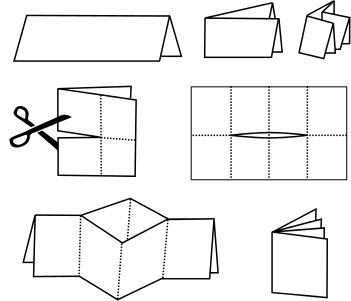
\includegraphics[width=.75\textwidth]{folding-minibook}}
%\date{Lycée Jean Zay}

%%%%%%%%%%%%%%%%%%%%%%%%%%%%

%%%%%%%%%%%%%%%%%%
\begin{document}
\maketitle
%---------------
\section{Diverses expressions}
\begin{center}
 \includegraphics[width=.92\textwidth]{pscalR1}
\end{center}
\newpage
%\rule{0pt}{1cm}
\begin{center}
 \includegraphics[width=.92\textwidth]{pscalR2}
\end{center}
\textbf{Al-Kashi:} \boxed{CB^2=AB^2+AC^2-2AB\times AC\times\cos(\widehat{BAC})}
\section{Exercices}
\exo{}
Déterminer par projection de l'un sur l'autre le produit scalaire des deux vecteurs dans chaque case. L'unité est le carreau.
\begin{center}
 \includegraphics[width=.9\textwidth]{pscalR4}
\end{center}
%%%%%%%%%%%%
\newpage
\exo{Deux projections}
$ABC$ est rectangle en $A$. L'unité est le carreau.\\
\begin{minipage}{0.6\linewidth }
\begin{enumerate}
%\item $\V{AB}\cdot\V{CA}=$
\item $\V{BC}\cdot\V{BA}=$
\item $BC=$
\item En déduire $BH$.
\end{enumerate}
\end{minipage}\hfill
\begin{minipage}{0.38\linewidth }
\includegraphics[width=\linewidth]{pscalR6}
\end{minipage}
%$\boxed{\vv{AB}\cdot \vv{AC}=-AB\times AH}$
\exo{}
$ABC$ est un triangle équilatéral de côté 6. \\Calculez
\PS{AB}{AC} et \PS{AB}{BC}. 
%--
\exo{}
$ABCD$ est un carré de côté 4 et de centre $O$, calculez les produits scalaires par la méthode de votre choix:
\begin{multicols}{3}
%\begin{small}
\begin{enumerate}
\item \PS{AB}{CD}
\item \PS{AB}{AC}
\item \PS{BA}{DA}
\item \PS{AC}{BD}
\item \PS{AD}{BC}
\item \PS{AD}{CD}
\item \PS{OC}{OB}
\item \PS{OA}{OC}
\item \PS{OB}{AD}
\end{enumerate}
%\end{small}
\end{multicols}
%%
\exo{}
On considère un triangle $ABC$ où:\\ 
$AB=5$ et $BC=6$  et $\widehat{ABC}=60$\degre.\\
%\begin{enumerate}
%  \item Faire une figure.
 % \item 
  Calculer $\vv{BA}\cdot \vv{BC}$.
  %\item 
 \\ En remarquant que $\vv{CA}=\vv{CB}+\vv{BA}$, calculer $\vv{CA}\cdot \vv{CB}$.
%
 % On remarquera d'abord que $\vv{CA}=\vv{CB}+\vv{BA}$.
%\end{enumerate}
%%
\newpage
\exo{R$\heartsuit$C}
Dans cet exercice on se place dans un repère orthonormé $(O,\vec{\imath},\vec{\jmath}\,)$%$\Oij$.

Soit $\Vu\covec{x}{y}$ et $\Vv\covec{x'}{y'}$.%$\Vu$ et $\Vv$ deux vecteurs de coordonnées 
\\\ding{172} En développant: $\Vu\cdot\Vv=(x\vec{\imath}+y\vec{\jmath})(x'\vec{\imath}+y'\vec{\jmath})$\\ établir la formule analytique du produit scalaire:
\[\boxed{\Vu\cdot\Vv=xx'+yy'}\]
\ding{173} \'Etablir cette même formule en partant de
\[\Vu\cdot\Vv=\frac12\Big( ||\Vu||^2+||\Vv||^2-||\Vu-\Vv||^2\Big) \]
Rappel: On sait que $||\Vu||=\sqrt{x^2+y^2}$
%-----
\exo{ Formule analytique: $\vec{u}\cdot\vec{v}=xx'+yy'$}
Calculer les produits scalaires suivants :
\begin{enumerate}
  \item $\vec{u}\cdot\vec{v}$ où $\vec{u}\covec{15}{-8}$ et $\vv{v}\covec{6}{9}$
  \item $\vec{s}\cdot\vec{t}$ où $\vec{s}\covec{-1}{-2}$ et $\vv{t}\covec{-3}{-4}$
  \item $\vec{a}\cdot\vec{b}$ où $\vec{a}\covec{\sqrt{3}-2}{6}$ et $\vv{b}\covec{\sqrt{3}+2}{1}$
  \item $\vec{c}\cdot\V{UV}$ où $\vec{c}\covec{\sqrt{6}}{2}$, $U(\sqrt{24}+5;1)$, $V(5;\sqrt{2})$
  \item $\vec{r}\cdot\V{AB}$ où $\vec{r}\covec{3}{7}$, $A(-1;2)$ et $B(-3;6)$
  \item $\V{CD}\cdot\V{MR}$ où $C(5;6)$, $D(-1;4)$, $M(3;7)$ et $R(8;9)$
  \item $\V{ST}\cdot\V{EF}$ où $E(0;1)$, $F(3;0)$, $S(8;8)$ et $T(5;5)$
\end{enumerate}
%%
\exo{}
On considère les points $A(1\ ;\ 3)$, $B(3\ ;\ 1)$, $C(-2\ ;\ -2)$, $D(13\ ;\ -5)$ et $E(4\ ;\ 3)$.
\begin{enumerate}
  \item Les droites $(AC)$ et $(AB)$ sont-elles perpendiculaires ?
  \item Même question pour :
  \begin{enumerate}
    \item $(AC)$ et $(BD)$
  \item $(BE)$ et $(CD)$
  \end{enumerate}
\end{enumerate}
%%
\exo{}

\begin{minipage}{0.65\linewidth }
$ABCD$ est un carré. \\
On note $I$  et $J$ les milieux respectifs de $[BC]$ et $[CD]$.  
\\ Prouver que $(AI)\bot(BJ)$.
\end{minipage}\hfill
\begin{minipage}{0.25\linewidth }
\includegraphics[width=\linewidth]{pscalR3}
\end{minipage}
%\newpage
\exo{R$\heartsuit$C}
Soit $\Vu$ et $\Vv$ deux vecteurs. 
\begin{enumerate}
\item En développant $(\Vu-\Vv)^2$ retrouver la formule: $\Vu\cdot\Vv=\frac12\Big( ||\Vu||^2+||\Vv||^2-||\Vu-\Vv||^2\Big)$.
\item Déterminer une formule analogue faisant intervenir $||\Vu+\Vv||^2$
\item Tracez un parallélogramme $ABDC$ où on note $\Vu=\V{AB}$ et $\Vv=\V{AC}$. Traduire les deux relations précédentes pour $\Vu\cdot\Vv$ avec les longueurs de la figure.
\end{enumerate}
%
\newpage
%
\exo{}
On considère un triangle $ABC$ où $AB=3$, $AC=2$ et $BC=\sqrt{7}$

Calculez \PS{AB}{AC}. En déduire $\widehat{BAC}$

%%
\exo{}
On considère un triangle $ABC$ avec:\\ $AB=2$, $AC=3$ et $BC=6$. 
Déterminer une valeur approchée des angles de ce triangle.
%
\exo{}
Soit $ABC$ un triangle quelconque établir une formule permettant de calculer $\widehat{BAC}$ en fonction des côtés du triangle.
%%
%\newpage
\exo{}
\begin{minipage}{0.50\linewidth }
On considère un triangle quelconque $ABC$, $I$ le milieu de $[AB]$ et les points $D$ et $E$ tels que les triangles directs $ACD$ et $CBE$ soient isocèles et rectangles en~$C$.  On veut prouver que: $(CI)\bot(ED)$
\end{minipage}\hfill
\begin{minipage}{0.47\linewidth }
\includegraphics[width=\linewidth]{pscalR5}
\end{minipage}

\begin{enumerate}
 % \item Quelle conjecture faire sur $(CI)$ et $(ED)$?
%On a tracé $(CI)$ la médiane issue de $C$ dans $ABC$.

  %Quelle droite remarquable de $DCE$ semble-t-elle également être ?
  \item Justifier que $\vv{CI}=\dfrac{1}{2}\vv{CA}+\dfrac{1}{2}\vv{CB}$.
  \item En déduire que: $\vv{CI}\cdot \vv{DE}=\dfrac{1}{2}\left(\vv{CA}\cdot \vv{CE}-\vv{CB}\cdot \vv{CD}\right).$
  \item Conclure.
\end{enumerate}
%%


\end{document}
